\section{Determinare la forza tra due fili paralleli percorsi da
	correnti stazionarie e discutere la relazione con la terza
	legge di Newton.}
Un filo rettilineo percorso da una corrente $I$ produce a una distanza $r$ una campo magnetico, il cui modulo \`e dato dalla seguente formula:
\begin{equation}
 	B = \mu_0 \frac{I}{2 \pi r}
\end{equation}
Le cui linee di forza sono circonferenze aventi centro \textbf{sull'asse del filo stesso} (Il verso \`e determinato dal \textbf{verso della corrente}, attraverso la regola della mano destra).\\
Se si fanno interagire due fili paralleli, accade che vi \`e una mutua interazione: 

\noindent\begin{minipage}{0.4\textwidth}
	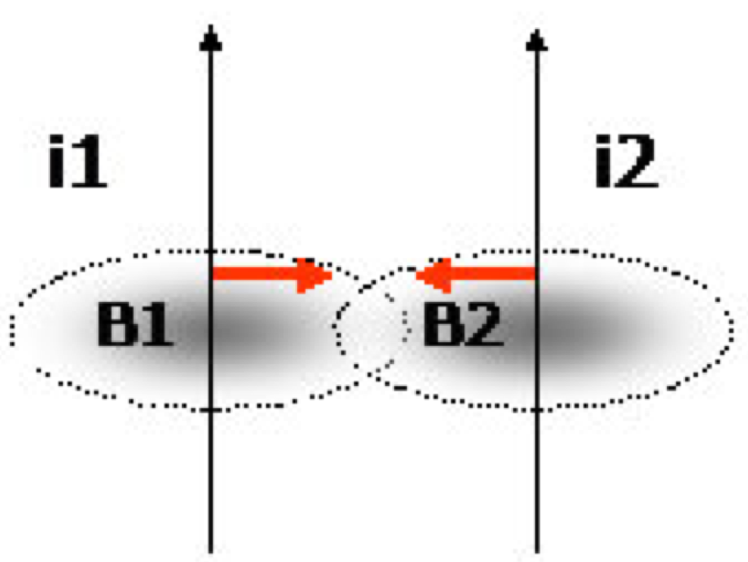
\includegraphics{fili_1}
\end{minipage}
\hfill%
\begin{minipage}{0.4\textwidth}\raggedleft
	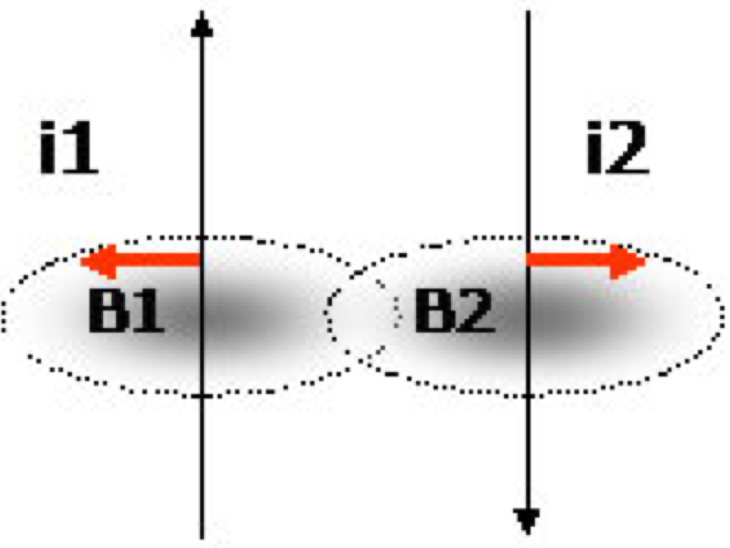
\includegraphics{fili_2}
\end{minipage}\\
 Sul filo 1 vi \`e una forza dovuta al campo $B_2$ mentre sul filo 2 vi \`e una forza dovuta a $B_1$. Si ha pertanto che:
 $$
     F_{1 \rightarrow 2} = B_2 I_1 d = \mu_0 \frac{I_2}{2 \pi d}I_1 = \mu_0 \frac{I_1 I_2}{2 \pi d}l
 $$
 $$
     F_{2 \rightarrow 1} = B_1 I_2 d = \mu_0 \frac{I_1}{2 \pi d}I_2 = \mu_0 \frac{I_1 I_2}{2 \pi d}l
 $$
 Dove $d$ \`e la distanza fra i due fili e $l$ \`e la lunghezza del tratto di filo considerato.\\
 La forza \`e attrattiva se i versi delle correnti sono \textbf{concordi}, mentre \`e repulsiva se sono \textbf{discordi}.
 Si noti che, proprio come in base alla Terza Legge di Newton, si ha che :
 $$
     \vec{F}_{1 \rightarrow 2} = -\vec{F}_{2 \rightarrow 1}
 $$
 $\hfill\square$